%%%%%%%%%%%%%%%%%%%%%%%%%%%%%%%%%%%%%%%%%%%%%%%%%%%%%%%%%%%%%%%%%%%%%%%%%%%%%%%%
%2345678901234567890123456789012345678901234567890123456789012345678901234567890
%        1         2         3         4         5         6         7         8

%\documentclass[letterpaper, 10 pt, conference]{ieeeconf}  % Comment this line out if you need a4paper

\documentclass[a4paper, 11pt, onecolumn, conference]{IEEEtran}      % Use this line for a4 paper

\IEEEoverridecommandlockouts                            %   This command is only needed if 
 % you want to use the \thanks command
\usepackage{graphicx}
\usepackage{float}
\usepackage[]{algpseudocode}
%\usepackage[]{algorithm2e}
%\usepackage[pdftex]{graphicx}

%\usepackage[final]{pdfpages}
%\usepackage[pdftex]{graphicx}
%\overrideIEEEmargins                                      % Needed to meet printer requirements.

% See the \addtolength command later in the file to balance the column lengths
% on the last page of the document

% The following packages can be found on http:\\www.ctan.org
%\usepackage{graphics} % for pdf, bitmapped graphics files
%\usepackage{epsfig} % for postscript graphics files
%\usepackage{mathptmx} % assumes new font selection scheme installed
%\usepackage{times} % assumes new font selection scheme installed
%\usepackage{amsmath} % assumes amsmath package installed
%\usepackage{amssymb}  % assumes amsmath package installed

\title{\LARGE \bf
ELEN4020A: Data Intensive Computing Laboratory Exercise No 1
}

\author{ Kopantsho Mathafa (849038)\ \ \ \ \ \ Chizeba Maulu (900968) \ \ \ \ \ \ 25 February 2019\\
}


\begin{document}

\maketitle

\section{Introduction}
Multidimensional arrays are common data structures in data intensive computing. Operations performed on these give rise to models in fields such as molecular biology and climate modelling. However, performing such operations requires a careful consideration of algorithm efficiency, accuracy and scalability. 
\\\\
This report discusses a study performed on 3 dimensional arrays, otherwise known as 3rd-order tensors. The study employs dynamically allocated $N$ x $N$ x $N$ arrays modelled in the Traditional Matrix Representation (TMR) form and applies matrix addition and multiplication operations to these arrays. The elements of these arrays are randomly generated integers valued between 0 and 20. To test for algorithm scalability, the array bound N is set at 10 and then at 20. Only the multiplication algorithm will be evaluated in this paper. 

\section{Background}
\subsection{Design Parameters and Success Criteria}

The approach employed for the 3-dimensional matrix multiplication algorithm is built upon the canonical 2-dimensional matrix multiplication algorithm. Equation 1 illustrates 2-dimensional matrix multiplication mathematically. 

\begin{equation}
    c_{ij} = \sum_{k} a_{ik} \times b_{kj}  
\end{equation}
Where: $a$, $b$ and $c$ - 2D Matrices and $i$, $j$, and $k$ - indices used to access the matrix elements. 
\\\\
Modifications are made to this well-known algorithm to account for the thired dimension in 3D matrices. \\\\
The TMR form of modelling an array is used. This was used both because of its flaws and merits. It is easier and more intuitive to model an array in TMR form as arrays in C as the array data structure is C is already in TMR form, even though in memory multi-dimensional arrays are stored as arrays of arrays instead of a single multidimensional structures.\\\\
The flaws of this form is the increase in both the cost of index computation and accessing or modifying the elements as the dimension of an array increases. These drawbacks allow for a better understanding of how algorithm efficiency can address the limitations of this kind of representation of arrays. \\\\
The requirements of the 3D multiplication algorithm and its results are:

\begin{itemize}
    \item It must be able to dynamically generate an array of integers.
    \item It must populate the array with randomly generated numbers between [0,20].
    \item Must be able to compute the multiplication of two 3-dimensional arrays.
    \item The program must store the result of the computation in a result matrix C with the correct array bounds in each dimensions, or as C[N][N]][N].
\end{itemize}

\subsection{3-Dimensional matrix multiplication algorithm}
In the design of the multiplication algorithm, the two 3D matrices are modelled as a 3D cube. This cube is then divided into sections which represent the 3 dimensions. This modelled is illustrated in Figure 1. All figures can be in the appendix.


Since the multiplication is now performed in 3 dimensions, instead of adding the products of row elements with column elements, it is necessary to compute the product of row- and column-planes. These planes are visualised in Figures 2 and 3.


Implementing this extraction of row plane and column planes, proved to be challenging. For this reason a further step was taken to divide the planes into column vectors and row vectors. This could be implemented by extracting elements using their indexed positions. A visual representation of this can be found in Figures 4 and 5.


Vector multiplication of each column and row block produce a single value, this is the value at the index where the row and column block intersect. For example, if we extracted the top row block and the leftmost column block, the matrix multiplication would be result in a value stored at Block 1 in Figure 1. This process is iterated through until the 3-dimensional result array is found.

\section{Critical Analysis and Future Recommendations}
The algorithm meets all the criteria outlined in section II. The accuracy of the results were confirmed manually using a scientific calculator. It was found that program correctly computed the multiplication.\\\\
The program could have been implemented to utilise parallel computing to make the computational efficiency higher. Parallel computing methods would have allowed for the use of other matrix models such the Extended Karnaugh Map Represenatation (EKMR).\\\\
The program is efficient, with regards to memory management. This is due to the use of \textbf{malloc()} and \textbf{calloc()}, which reserves only the required heap memory. \\

Pseudo code of the different functions can be found in the Appendix.

\section{Conclusion}
This report presents the 3D matrix multiplication algorithm designed, implemented and tested. The matrices were modelled in the Traditional Matrix Representation. The elements of these matrices were randomly generated to be between 0 and 20. The algorithm computed the products of two 3D matrices with bounds 10 and 20. The algorithm performed the products accurately. 

\newpage
\appendix

\begin{algorithmic}

\Function{createArray}{$dimension$}

\For{$row=0$;  $row \gets dimension$}
    \For{$column=0$; $column \gets dimension$}
        $matrix[row][column] = rand() \% 21$
    \EndFor
\EndFor
\EndFunction \\ \\


\Function{rank2TensorAdd}{$A, B, rank$}
\For{$row=0$; $row \gets rank$}
    \For{$column=0$; $column \gets rank$}
        $result[row][column] = A[row][column] + B[row][column]$ 
    \EndFor
\EndFor
\EndFunction \\ \\ 

\Function{rank2TensorMult}{$A, B, rank$}
\For{$row=0$; $row \gets rank$}
    \For{$column=0$;  $column \gets rank$}
        \For{$iterator=0$; $iterator \gets rank$}
        $result[row][column] += A[row][iterator] + B[iterator][column]$ 
        \EndFor
    \EndFor
\EndFor
\EndFunction \\ \\

\Function{printFunc}{$matrix,size$}
\For{$row=0$; $row \gets size$}
    \For{$column=0$;  $column \gets size$}
        $print(matrix[row][column])$
    \EndFor
\EndFor
\EndFunction \\ \\

\Function{rank3TensorMult}{$A$,$ B$,$rank$}

\For{$depth=0$; $depth \gets rank$}
    \For{$row=0$;  $row \gets rank$}
        \For{$column=0$; $column \gets rank$}
            \For{$iterator=0$;  $iterator \gets rank$}
                 $result[row][column][depth] += A[row][iterator][depth] + B[iterator][column][depth] $
            \EndFor
        \EndFor
    \EndFor
\EndFor

\EndFunction \\ \\ \\ 

\Function{rank2TensorAdd}{$A, B, rank$}
\For{$depth=0$; $depth \gets rank$}
    \For{$row=0$;  $row \gets rank$}
        \For{$column=0$; $column \gets rank$}
      $$  result[row][column][depth] = A[row][column][depth] + B[row][column][depth] $$
        \EndFor
    \EndFor
\EndFor
\EndFunction \\ \\

\end{algorithmic}

\begin{figure}[H]
\centering
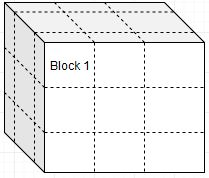
\includegraphics[width=0.4\textwidth]{MatrixBlock.JPG}% graph
\caption{Divided 3D Cube}
\label{fig:1}
\end{figure}

\begin{figure}[H]
\centering
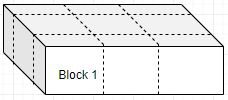
\includegraphics[width=0.35\textwidth]{VPlaneBlock.JPG}% graph
\caption{Row Plane}
\label{fig:2}
\end{figure}

\begin{figure}[H]
\centering
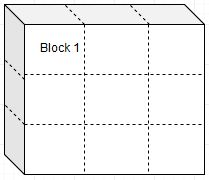
\includegraphics[width=0.35\textwidth]{MatrixPlane.JPG}% graph
\caption{Column Plane}
\label{fig:3}
\end{figure}

\begin{figure}[H]
\centering
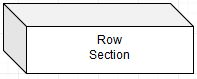
\includegraphics[width=0.35\textwidth]{RowBlock.JPG}% graph
\caption{Row Block}
\label{fig:4}
\end{figure}

\begin{figure}[H]
\centering
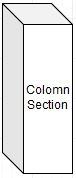
\includegraphics[width=0.1\textwidth]{ColomnBlock.JPG}% graph
\caption{Column Block}
\label{fig:5}
\end{figure}


\end{document}

